\documentclass{article}
\usepackage[utf8]{inputenc}
\usepackage{graphicx}
\usepackage{url}
\usepackage{xcolor}
\usepackage{listings}
\lstset{basicstyle=\ttfamily,
  showstringspaces=false,
  commentstyle=\color{red},
  keywordstyle=\color{blue}
}
\usepackage[margin=1.5cm]{geometry}


\title{A short hands on RAMSES}

\author{Ugo Lebreuilly & Beno\^it Commer\c con}
\date{}
\begin{document}
\maketitle


\section{Quick start}
\subsection{First compilation}

Let's start by cloning RAMSES in the desired directory
\begin{lstlisting}[]
$ git clone https://bitbucket.org/rteyssie/ramses
\end{lstlisting}
Then for a quick compilation
\begin{lstlisting}[]
$ cd ramses/bin 
$ make
\end{lstlisting}
You now have an executable for RAMSES (ramses1d). This is the default executable, it is not usable for every setup. We are now going to see what kind of things we can typically change with the makefile. 
\subsection{Makefile}
Open the Makefile file (still in the bin) with your favorite text editor. As you can see there are plenty of pre-compilers that you can change (for example DEBUG, COMPILER etc...) to get a different executable (adapted to the problem that you want to run). Here we compiled the code with the hydro solver (i.e. without magnetic field, you can change that by modify the SOLVER pre-compiler to SOLVER =mhd). We compiled in 1D, so you have to put NDIM = 3 if you want for example to do a 3D calculation. 
\section{Tests}
\subsection{Test suite}

As you can see there is a PATCH pre-compiler that has no default value, this is the one that you want to modify if you have a particular setup in mind. This is will be important soon, let's keep that in mind while going to the tests folder.  
\begin{lstlisting}[]
$ cd ../tests
\end{lstlisting}
You see several folders here, corresponding to tests that are run on a daily basis to verify the well being of RAMSES. There is run\_test\_suite.sh file in the folder. You can simply execute it like that
\begin{lstlisting}[]
$ ./run_test_suite.sh -t 1
\end{lstlisting}
You will only run test 1 which is called hydro barotrop. Once the test is performed it should create a file name test\_results.pdf. Open it and if the test was successful you should see something like in figure 1.
\begin{figure}[h!]
\centerline{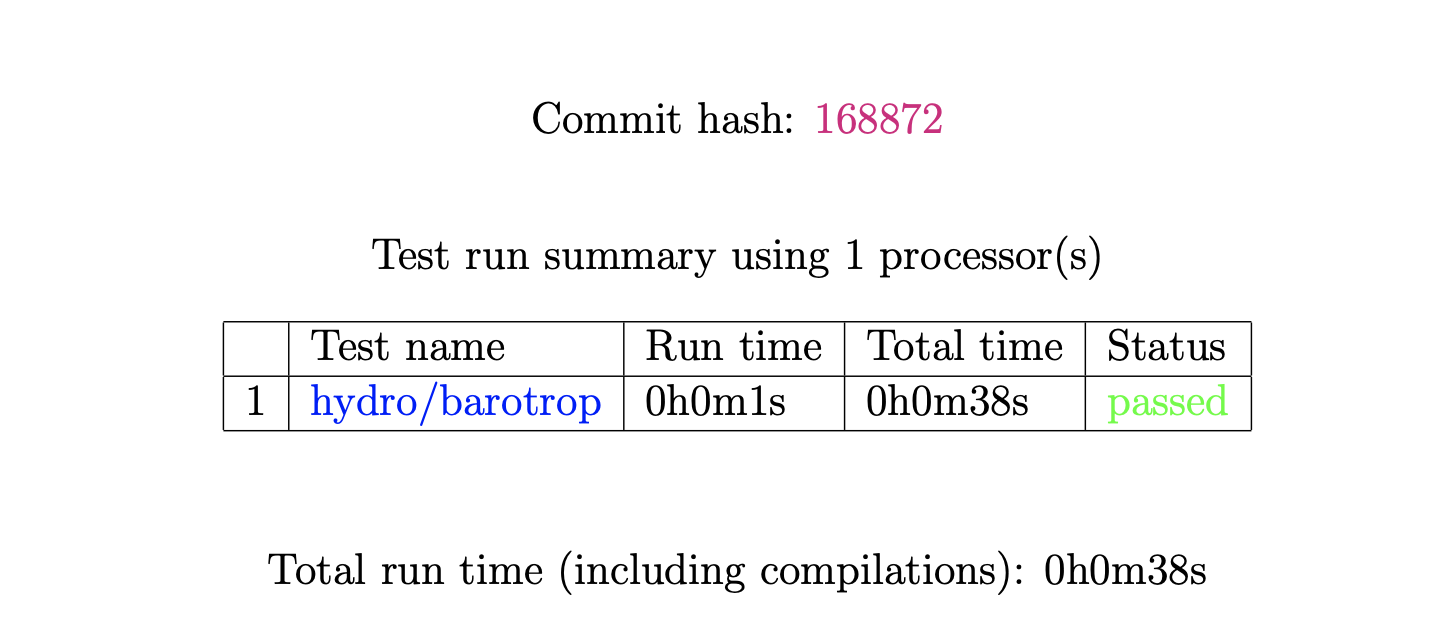
\includegraphics[width=\textwidth]{figures/test_success.png}}
\caption{Summary of the barotrop test in case of success.}
\end{figure}
Here we see that we have run successfully the barotrop test in 38s (including the compilation time because the run time was only 1s). We can also this that we have run the RAMSES version corresponding to the commit 168872. We can see in figure 2 the results of the run 
\begin{figure}[h!]
\centerline{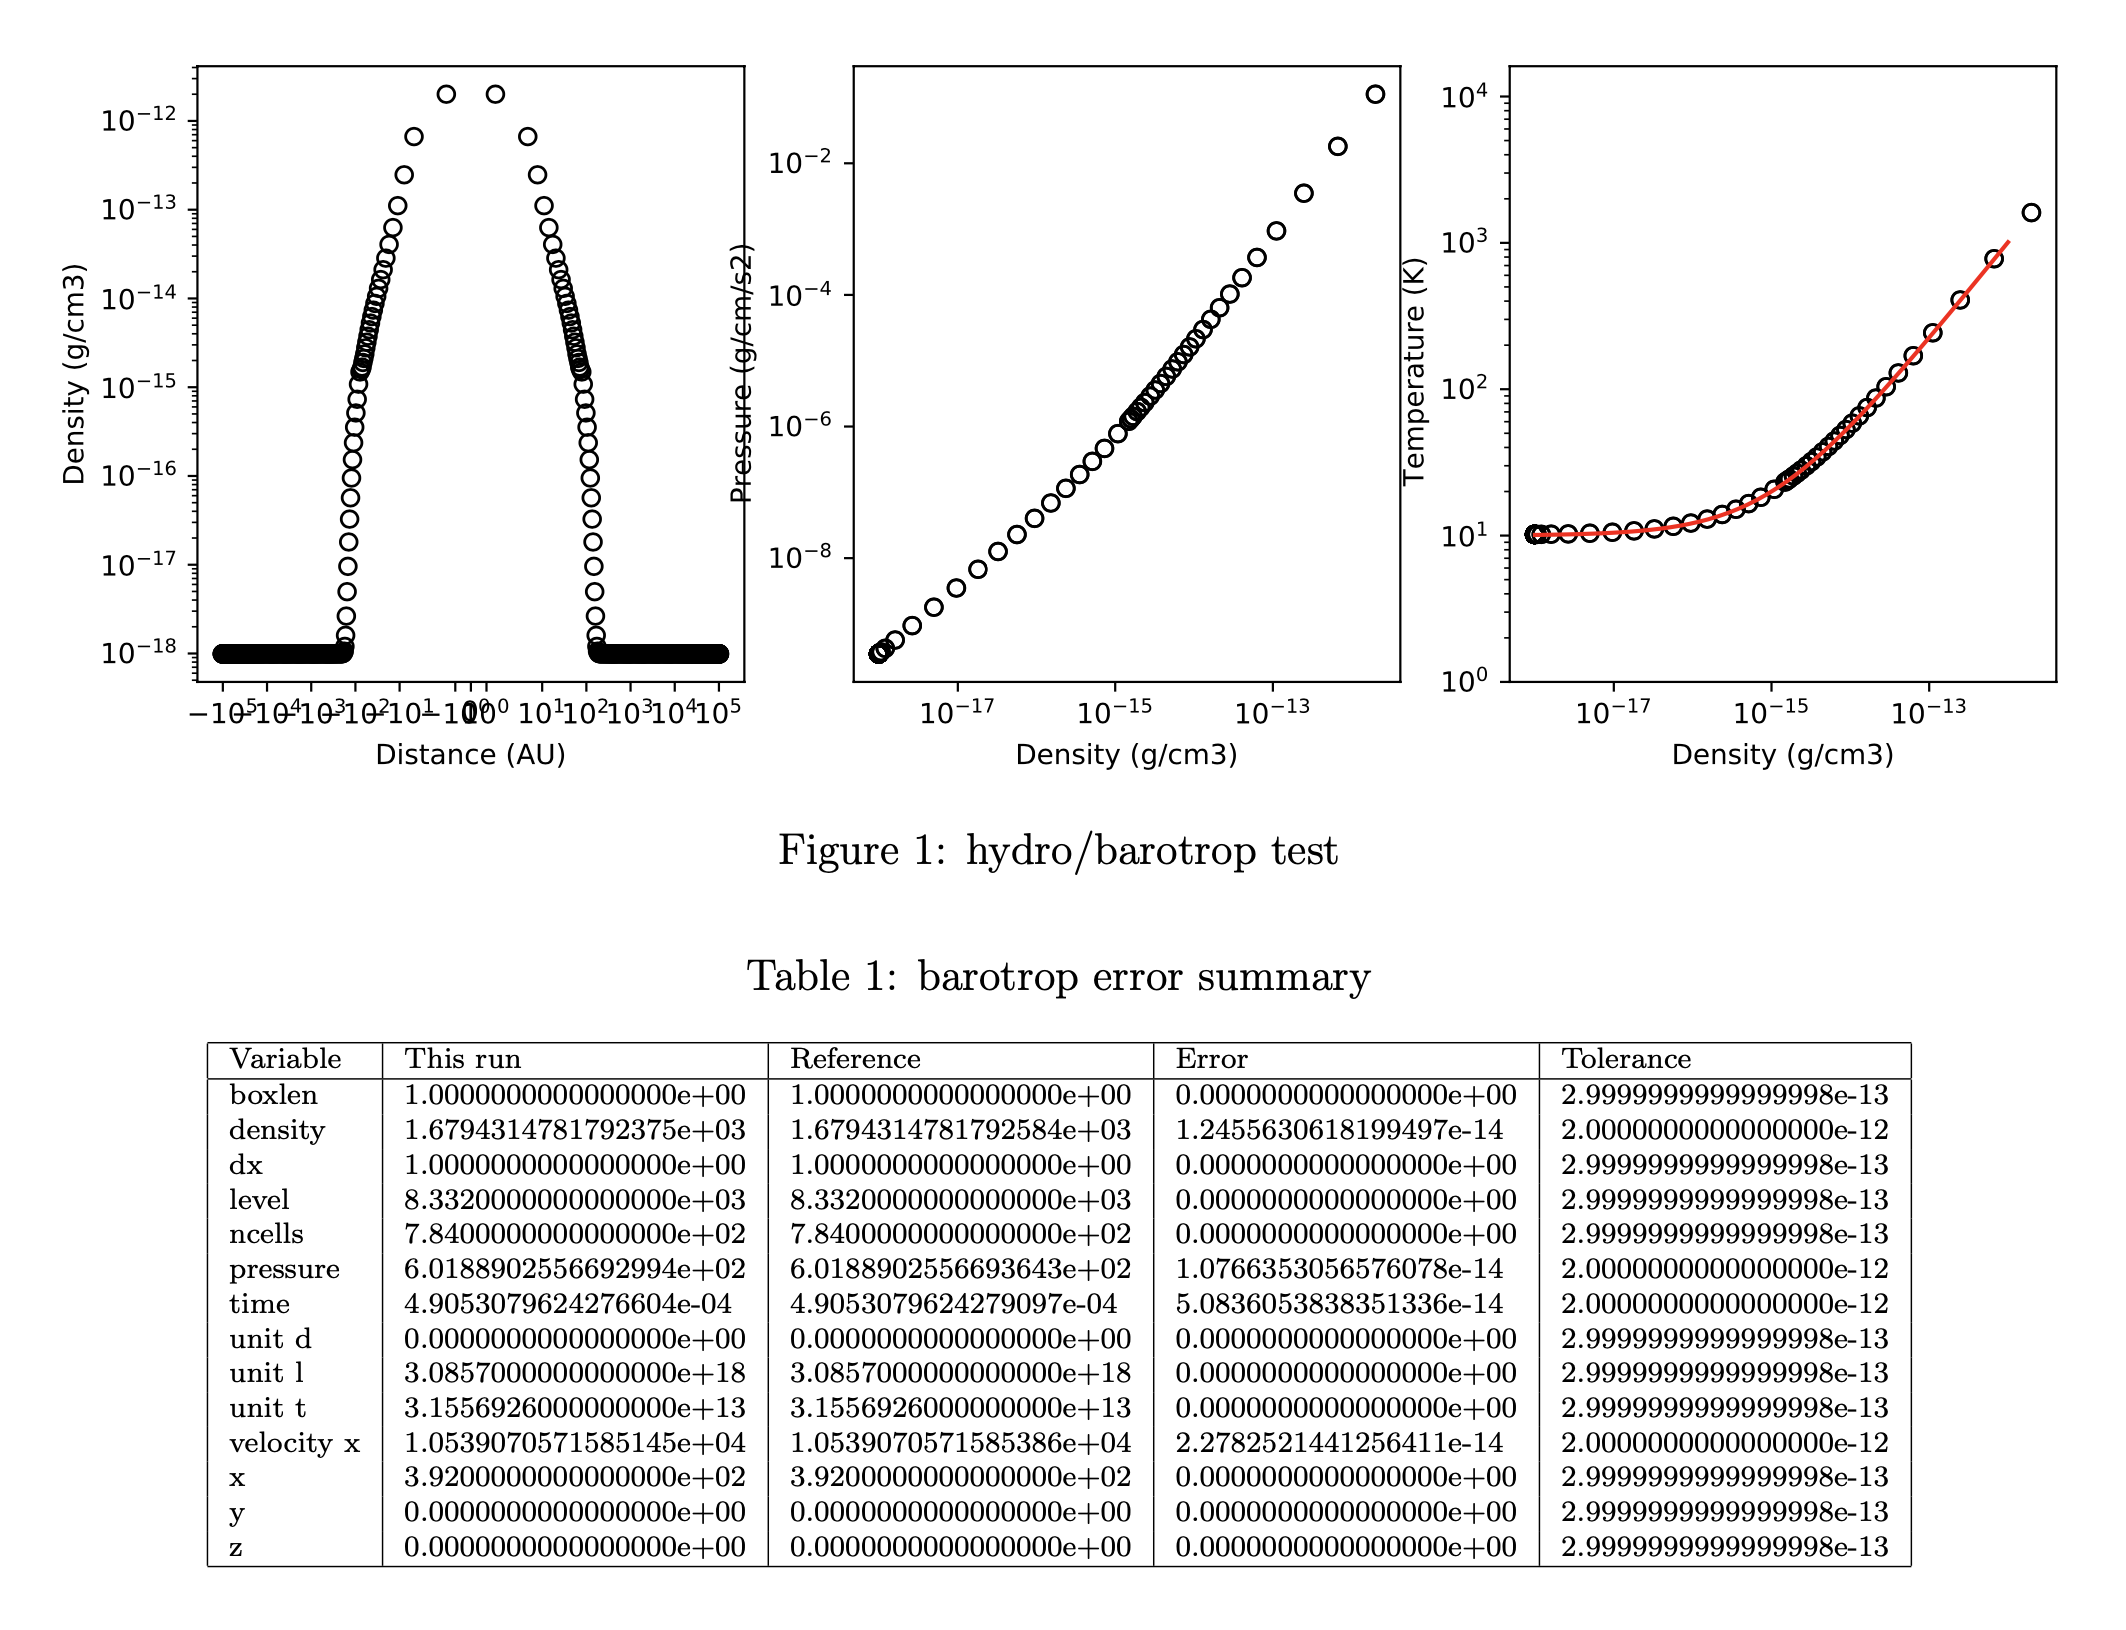
\includegraphics[width=\textwidth]{figures/barotrop.png}}
\caption{Results of the barotrop test. Top: Density plots. Bottom: Table that compares the results with the reference solution.}
\end{figure}

Note that here we have run only the test #1, but there are more. In fact
12 tests are run by the RAMSES code on a daily basis. 
\begin{lstlisting}[]
 [ 1] hydro/barotrop
 [ 2] hydro/cooling-frig
 [ 3] hydro/implosion
 [ 4] hydro/isothermal
 [ 5] hydro/sod-tube
 [ 6] mhd/imhd-tube
 [ 7] mhd/orszag-tang
 [ 8] rt/stromgren2d
 [ 9] sink/levelhack
 [10] sink/smbh-bondi
 [11] turb/driving
 [12] tracer/sedov
\end{lstlisting}
If you now execute again the run\_test\_suite.sh file but without any argument, then you will run all the tests... but let's not do that.
We will now aim to run a test without the help of the run\_test\_suite.sh file.

\subsection{Running our own setup}
We have seen how to use the test suite, but this is simpler that running a custom calculation as all is automatise. Now, let’s try to redo the sedov test but all by ourserlves !

Lets go inside the sedov folder located in the tracer folder of the tests directory. 
\begin{lstlisting}[]
$ cd tracer/sedov
\end{lstlisting}
There should be at least 4 files in the directory.We are particularly interested with 2 of them. A config.txt file that gives the compiling information to run the test and a a namelist file called sedov.nml were the parameters of the run are given. 
If we open the config.txt file we see that it contains only one line 
\begin{lstlisting}[]
FLAGS: NDIM=2 PATCH= SOLVER=hydro
\end{lstlisting}
This gives the pre-processors that need to be modified from the by-default Makefile of ramses in order to run the test. Here the sedov tests is run in 2D, without any PATCH (we will explain what those are after) and with the hydro solver (the other solver of ramses is the mhd solver).

We will now compile the code with this configuration, let's go back to the bin folder 
\begin{lstlisting}[]
$  cd ../../../bin
\end{lstlisting}
You can modif the makefile to give the preprocessors the values of the config.txt file or you can simply run 
\begin{lstlisting}[]
$ make NDIM=2 PATCH= SOLVER=hydro
\end{lstlisting}
This is quite convenient because we kept the makefile unchanged (to the default version). Running this command should have compiled the code and made a executable that is suited for the sedov test. Since we compile the code in 2D, the executable is called ramses2d. You can copy it in a sedov-test folder that you can create wherever you can. Then also copy the namelist file that was in the sedov test folder and go in the directory 
\begin{lstlisting}[]
$ cp ../tests/tracer/sedov/sedov.nml /your/directory/sedov-test/.
$ cd /your/directory/sedov-test/
\end{lstlisting}
We have now everything to run the test here. This can be simply achieved by the command 
\begin{lstlisting}[]
$ ./ramses2d sedov.nml
\end{lstlisting}

Note that we indicated ramses2d that it should read its parameters in the namelist (sedov.nml) file. While the code is running you can open the file to see what's inside.
It should look like that
\begin{lstlisting}[]

&RUN_PARAMS
hydro=.true.
pic=.true.
tracer = .true.
ncontrol=1
nrestart=0
nremap=0
nsubcycle=10*2
/

&AMR_PARAMS 
levelmin=5
levelmax=7
ngridtot=50000
nparttot=500000
nexpand=1
boxlen=0.5
/

&INIT_PARAMS
nregion=2
region_type(1)='square'
region_type(2)='point'
x_center=0.5,0.0
y_center=0.5,0.0
length_x=10.0,1.0
length_y=10.0,1.0
exp_region=10.0,10.0
d_region=1.0,0.0
u_region=0.0,0.0
v_region=0.0,0.0
p_region=1e-5,0.4
/

&OUTPUT_PARAMS
foutput=100000
noutput=2
tout=0.0,1.0
/

&HYDRO_PARAMS
gamma=1.4
courant_factor=0.8
scheme='muscl'
slope_type=1
/

&REFINE_PARAMS
err_grad_d=0.01
interpol_type=1
/


&tracer_params
MC_tracer = .true.
tracer_feed_fmt = 'inplace'
tracer_mass = 1e-6
/
\end{lstlisting}

As you can see several parameters are set and there are arranged in different categories : RUN\_PARAMS,  AMR\_PARAMS,  INIT\_PARAMS,  OUTPUT\_PARAMS,  HYDRO\_PARAMS,  REFINE\_PARAMS and  TRACER\_PARAMS. Each of these categories corresponds to different parts of the code. For example INIT\_PARAMS corresponds to the initial conditions, AMR\_PARAMS to the grid properties and REFINE\_PARAMS to the criterion for refining the grid. Here it becomes pretty clear, that by modifying the namelist you can change what ramses is doing. For example we could change boxlen to 1 to make a sevod blast with a box of size 1. 

By now the test should be over. There should be two output folders in the directory. output\_00001 corresponds to the initial state and output\_00002. If you go inside of these folder you see a lot of files, but nothing easy to read. We now need a post-processing tool to be able to read the data created by ramses.
\section{Reading the data}

There are several post-processing tools out there to read RAMSES data, like Osyris, PYMSES or YT (among others). 
We are going to use Osyris, available here \url{https://github.com/osyris-project/osyris}. You can see that there is plenty of documentation over there. We are going to review the basics. 
You can install osyris with pip like that 
\begin{lstlisting}[]
$ pip install osyris
\end{lstlisting}
Note that we also need thre pint package that deals with physical units. 
\begin{lstlisting}[]
$ pip install pint
\end{lstlisting}
If can now import the osyris package with python. Open a python shell in the directory where you outputs are an type
\begin{lstlisting}[]
$ import osyris
$ import matplotlib.pyplot as plt
$ import numpy as np
\end{lstlisting}
You can now read the output 2 with the command 
\begin{lstlisting}[]
$ data = osyris.Dataset(2).load()
\end{lstlisting}
Note that the command 
\begin{lstlisting}[]
$ data = osyris.Dataset(-1).load()
\end{lstlisting}
would also work, the first argument of the function Dataset can be set to -1 to read the last output of the folder. We can now plot our data. If we for example want to do a density slice, we can run the following command.
\begin{lstlisting}[]
$ osyris.map({"data": data['hydro']["density"], "norm": "log"}, cmap='jet')
$ plt.show()
\end{lstlisting}
Here we have done a log-scaled density slice. There are plenty of other things that OSYRIS is able to do, we suggest that you play with it for a while. You can for example try to plot histograms or directly play with the data using numpy. You can take a look at the documentation of OSYRIS at the following link \url{https://osyris.readthedocs.io/en/stable/}.

\section{Patches}

We are now going to be diving into the patches, which are very useful ways to modify the code in order to obtain the desired behaviour. We are going to review these patches by trying to run a protostellar collapse calculation. Now go back to the ramses repository and go in the coeur patch.
\begin{lstlisting}[]
$ cd patch/mhd/coeur
\end{lstlisting}

If you ls this patch you while see 6 files
\begin{lstlisting}[]
barotrop.nml		condinit.f90		cooling_fine.f90

hydro_parameters.f90	read_hydro_params.f90	units.f90
\end{lstlisting}
There is a namelist, that will be used the same way as for the sedov test. But there are also f90 files. For example condinit.f90, specifies the initial conditions of the problem and units.f90 its units. Note that these two files are modifications of files that are already present in RAMSES. That is precisely the point of patches, if a setup requires modification in a few files of RAMSES, and if these modifications would break the rest of the code (for example if you change the units), then you can copy f90 files into the patch and modify them here. Note that it is better if you copy the least number of file as possible to manage the patch and keep compatibility with the main code more easily.  

Now if you compile the code without changing the makefile the main versions of condinit.f90 and units.f90 will be compiled and you wont be able to run a collapse test. To compile with the coeur patch go back to the bin folder, clean it with the command
\begin{lstlisting}[]

$ make clean

\end{lstlisting}
And now compile it like that 
\begin{lstlisting}[]
$ make NDIM=3 PATCH=../patch/mhd/coeur SOLVER=mhd NDIM=3
\end{lstlisting}
You have now a ramses3d executable that can be used to run collapse calculations (using the barotrop.nml namelist). Now we would like to use ramses parallelisation in order to run it faster. It is possible to compile with open mpi again using preprocessors
\begin{lstlisting}[]
$ make clean
$ make NDIM=3 PATCH=../patch/mhd/coeur SOLVER=mhd NDIM=3 MPI=1
\end{lstlisting}

Now copy the executable and the namelist file into  collapse-run directory when you want to run the simulation. Once it's done you can go in this directory. Let's assume you want to run the code with 4 CPUs, then the command is simply 
\begin{lstlisting}[]
$ mpirun -np 4 ramses3d barotrop.nml
\end{lstlisting}
Note that you can keep the terminal information in a log file (e.g. collapse.log) with the command 
\begin{lstlisting}[]
$ mpirun -np 4 ramses3d barotrop.nml > collapse.log
\end{lstlisting}

\section{Practical work : A collapse calculation}

\begin{figure}[h!]
\centerline{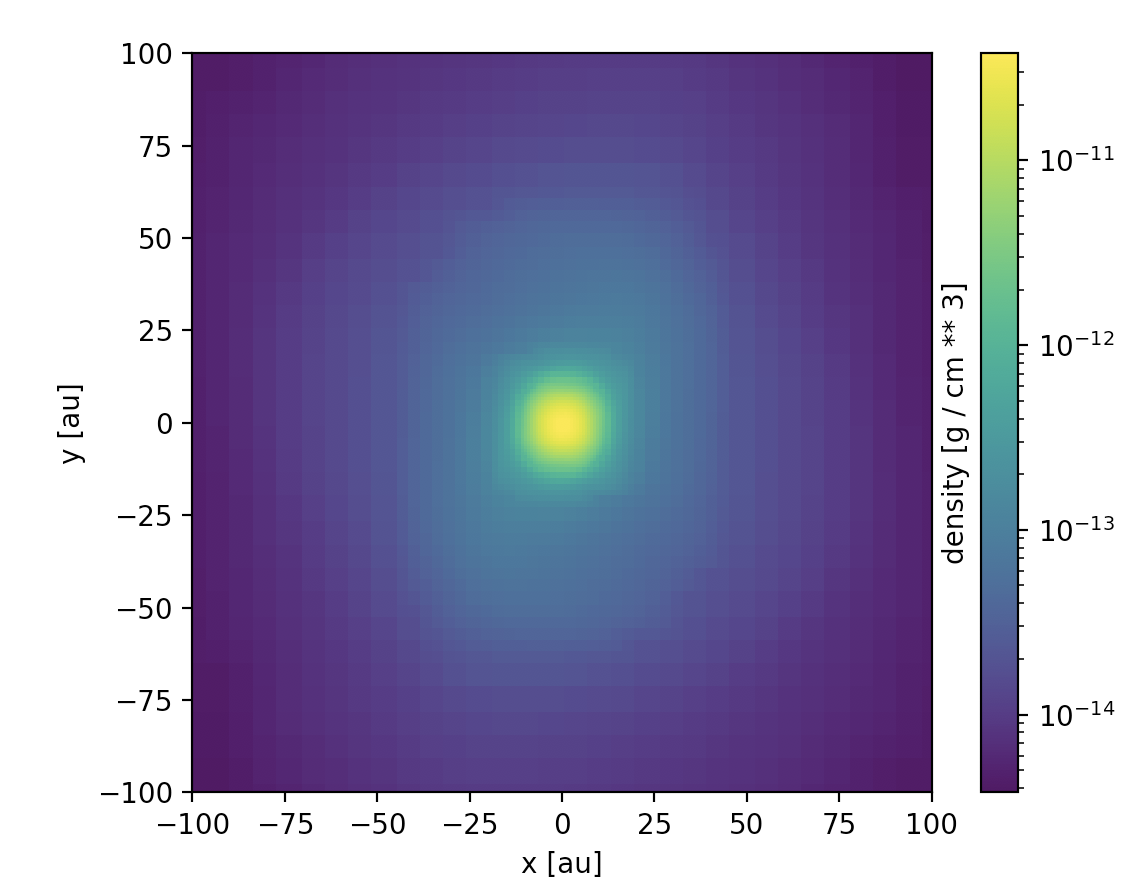
\includegraphics[width=0.4\textwidth]{figures/slice_20.png}}
\caption{Slice of 200 au x 200 au in the z direction obtained with OSYRIS for the snapshot 20 centered at the position of the density maximum.}
\end{figure}
Let's now run a collapse calculation with the aim of writing a python pipeline to analyse it. The goal of this exercise is to write a scripts that analyses every output of the simulations. For each snapshot we will compute
\begin{itemize}
    \item a slice of the density and temperature in the x, y and z directions
    \item a density PDF to learn how to handle the raw data that are read by OSYRIS.
\end{itemize}
To perform this analysis we will use the documentation of Osyris (available at \url{https://osyris.readthedocs.io/en/stable/}).
In addition, if we have time we can start to extract structures (such as the first core). When the density reaches values higher than $10^{-11}~$g cm$^{-3}$, fragments called first Larson cores are forming. We propose to measure the mass as a function of time. This will require to filter the data with masks (using the criterion $\rho>10^{-11}~$g cm$^{-3}$) and to perform the mass measurement on these filtered data.

\section{Run on mesopsl}
Below are the instruction to run RAMSES on mesopsl.

Clone RAMSES on your home directory 
\begin{lstlisting}[]
$ git clone https://bitbucket.org/rteyssie/ramses.git
\end{lstlisting}

Load the modules to compile RAMSES with fortran and MPI
\begin{lstlisting}[]
$ module load gcc 
$ module load openmpi
\end{lstlisting}

And compile the code
\begin{lstlisting}[]
$ cd ramses/bin/
$ make NDIM=3 PATCH=../patch/mhd/coeur SOLVER=mhd NDIM=3 MPI=1
\end{lstlisting}

We will now run RAMSES on the /travail scratch disk space and copy the executable and namelist files
\begin{lstlisting}[]
$ cd /travail/yourlogin/
$ cp ~/ramses/bin/ramses3d .
$ cp ~/ramses/patch/mhd/coeur/barotrop.nml .
\end{lstlisting}

Example of submission script
\begin{lstlisting}[]
#!/bin/sh
#SBATCH --job-name=test
#SBATCH --time=00:01:00
#SBATCH --mail-user=your.email --mail-type=ALL
#SBATCH --clusters=astro_thin
#SBATCH --partition=def
#SBATCH --qos=astro_thin_def_long
#SBATCH --account=formation
#SBATCH --nodes=1
#SBATCH --ntasks-per-node=24

module load gcc
module load openmpi

RUNDIR=/travail/yourlogin/test/
cd ${RUNDIR}

mpirun -np ${SLURM_NTASKS} ramses3d barotrop.nml


exit 0
\end{lstlisting}

To do visualisation and analysis, install OSYRIS

\begin{lstlisting}[]
$ module load python
$ pip install ipython
$ pip install osyris
\end{lstlisting}


\end{document}